\documentclass[english]{article}

%% Packages pull in extra commands:
%% http://en.wikibooks.org/wiki/LaTeX/Packages
\usepackage[latin9]{inputenc}
\usepackage[letterpaper]{geometry}
\usepackage{pgfplots}
\usepackage{graphicx}
\graphicspath{ {imgs/} }
\geometry{verbose,tmargin=1in,bmargin=1in,lmargin=1in,rmargin=1in}

\title{CIS 520 Project Final Report: Twitter Gender Classification}
\author{Woodpecker (Xiang Deng, Yiren Lu, Dongni Wang)}
\date{Fall 2015}

\begin{document}
\maketitle
For the final project, we developed a system for gender prediction (male/female) from the language of their tweets and their profile images. We were given a training set of 4998 labeled training samples and a testing set of 4997 testing samples. Each sample has 5000 words features, 7 pre-extracted image features and 30000 raw RGB image pixel features. The time constraint for initializing the model(s) is 3 minutes, for final prediction is 10 minutes for 5,000 test samples and the submission size is limited to 50 Mb in the final checkpoint competition. Our submitted model for the final competition achieved an accuracy of 91.04\% on the validation set, ranked $6^th$ in a total of 50 2-3 people teams. \par
In our system, we used seven classifiers on different feature sets and combined them using the stacking method.
The seven classifier are: a logistic regression model on words features, an ensemble model consists of 300 decision stump trees using LogitBoost on selected words and image features, a SVM model with intersection kernel on selected words and image features, a SVM model with intersection kernel on selected and normalized words and image features, an ANN model with 2 hidden layers each with 100 and 50 nodes, a SVM model with RBF kernel on PCA-ed HOG features on face-detected images, and a SVM model with RBF kernel on PCA-ed LBP features on face-detected images. For the stacking method, we took the raw outputs (probabilities) from the seven basic models mentioned above trained with 80\% of training samples and trained a logistic regression model using the other 20\% of training sample. Our final full model achieved an overall accuracy of 92.42\% on testing set. \par
 In order to meet the time and space constraint for the competition, we dropped the SVM model on PCA-ed LBP features and replaced the SVM model on PCA-ed HOG features with one bagging of logistic regression classifiers on raw HOG features. \par
In the following sections, we present the cross-validation accuracies of each methods we tried and discuss the rationale of our final model. We also provide some interesting visualization such as the most predictive words and the visualization of auto-encoder.  

\begin{center}
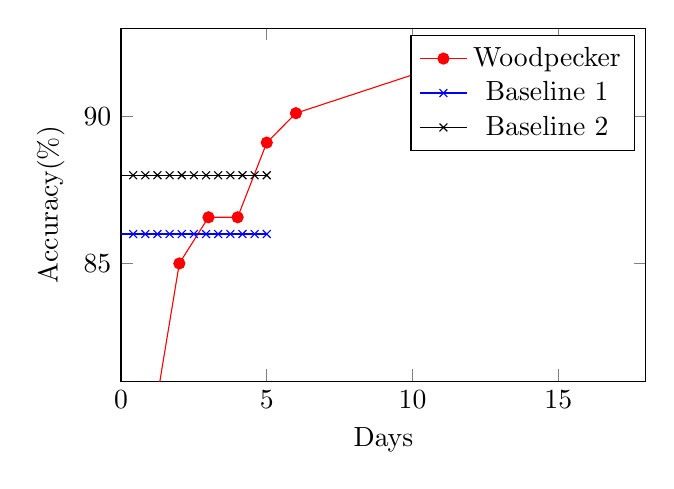
\begin{tikzpicture}
  \begin{axis}[
  		width=0.68\textwidth,
      	height=0.5\textwidth,
		xlabel={Days},
		ylabel= Accuracy(\%),
      	xmin= 0,
      	xmax= 18,
      	ymin=81,
      	ymax=93],
	\addplot[color=red,mark=*] coordinates {
		(1,79)
		(2,85)
		(3,86.57)
		(4,86.57)
		(5,89.11)
		(6,90.11)
		(11,91.74)
		(12,91.9)		
		(15,92.3)
		(17,92.42)
	};
	\addplot[color=blue,mark=x]{86};
	\addplot[mark=x]{88};

\legend{Woodpecker,Baseline 1, Baseline 2}
	\end{axis}
\end{tikzpicture}
\end{center}


\section{Methods}
In this section, we report the results of multiple methods we tried for feature extraction, dimension reduction, and classification. 

\subsection{Data Preprocessing}
\subsubsection{Stemming and Stop Words}
Conclusion: Did not work!

\subsection{Feature Selection}
To extract features from the raw word and image features, we experimented with multiple feature selection methods, including Information Gain, BNS
\subsubsection{Information Gain Over Words Features}
words visualization
\subsection{Dimension Reduction}
\subsubsection{PCA}

\subsection{Classification on Words Features and Extracted Image Features}
\subsubsection{Linear Regression (L2 Regularization) + Sigmoid}
\subsubsection{Logistic Regression + PCA}
\subsubsection{Logistic Regression on Raw Features}
\subsubsection{Naive Bayes}
\subsubsection{Neural Network}
\subsubsection{LogitBoost and Feature Selection Using Information Gain}
 We want to use both words features and image features in order to enhance our accuracy, but we don't know which feature is most informative; therefore, we ranks all words and image features together using information gain and select the top features (In fact, by computing the information gain of image features, we found image feature 1 2 5 6 and 7 have roughly 0 information gain, but of course this does not mean all image features are useless).\\
On the other hand, Logitboost can be seen as a convex optimization which combines Adaboost with the cost function of logistic regression. We experiments with Logitboost based on the following considerations.\\
1. Words and the seven image features have different scales, we need a model that is scale invariant; boosting with decision stump trees in this case is a great choice.\\
2. The cost function using logistic regression is suitable for binary classification, it is a convex problem and minimizes the binomial deviance and gives less weights to misclassified observations.\\
By selecting the top 1000 features ranked by information gain and using 330 decision stump trees, we achieved an accuracy of 89.11 percent on the testing set.\\
In our final submission, this model also serves as a major classifier that contributes to our ensemble method.\\
Below is the cross validation accuracy plots (over 8 folds):\\
\begin{center}
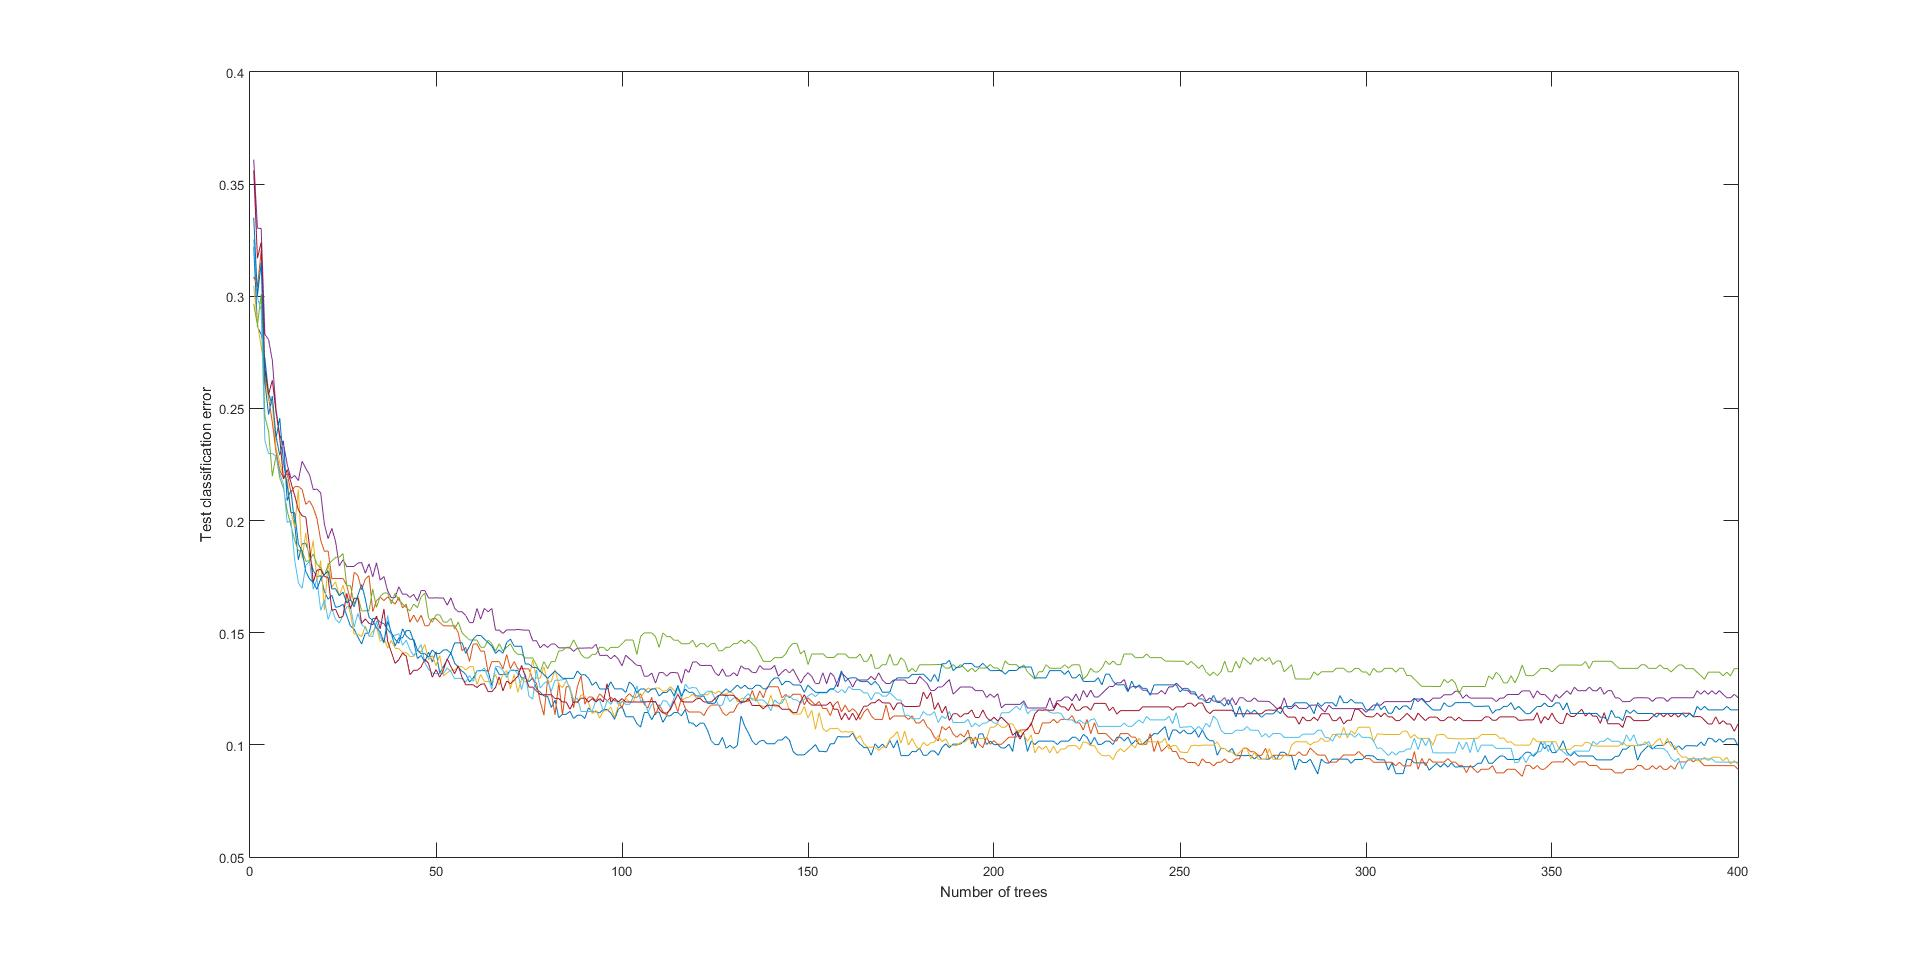
\includegraphics[scale=0.25]{logitboost.jpg}
\end{center}
\subsubsection{Kernel SVM}
\subsection{Classification on Image Features}
\subsubsection{Grey-scale Images}
We first converted the profile images data into R, G, B and Grey-scale images. 
\subsubsection{Face Detection with Viola-Jones Algorithm}
We extracted all the faces. We used matlab built-in Viola-Jones algorithm to do face detection on RGB images, which detected faces on 72\% of the profile pictures. All the following classifications over images were based on the faces detected. Later when ensemble, we only used samples with detected faces. For those samples without faces in them, we just set the output of the classifier as 0 (the output of the classifier is either positive or negative for male or female).
\subsubsection{Logistic Regression with Eigen Faces}
After extracted faces, we did PCA over grey-scale images, the visualization of the top principal components are shown in figure below. We put top PCs into logistic regression classifier and it yielded 60+\% accuracy. \\
\begin{center}
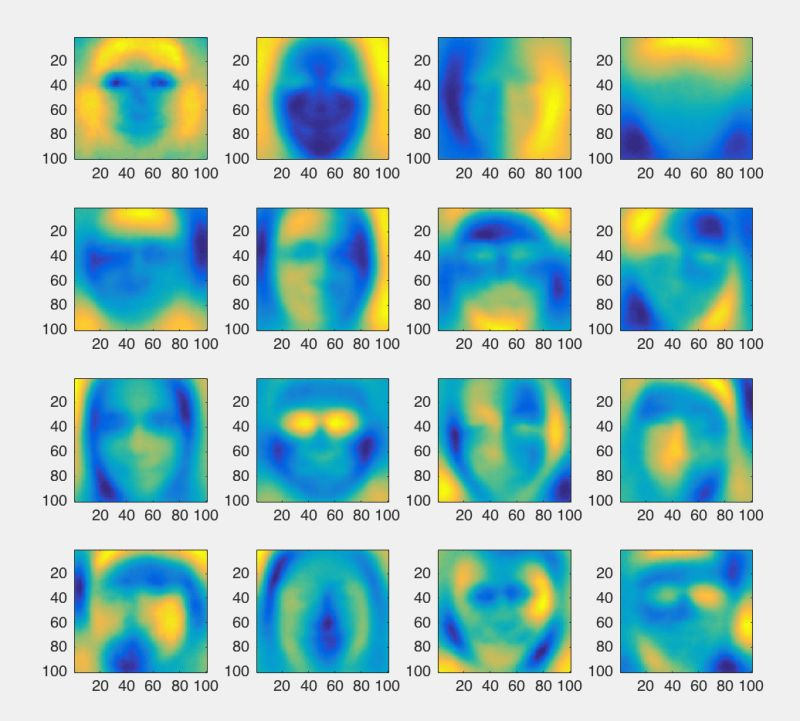
\includegraphics[scale=0.5]{pca_faces}
\end{center}
\subsubsection{HOG Features, Gaussian Pyramid, Eyes and Nose}
We used Viola-Jones algorithm to detect and crop eyes and nose. After that, we extracted Gaussian Pyramid HOG features into 7020 feature vector. Classifying the features with logistic regression yielded 82\% accuracy by itself on 72\% detected faces. The ensemble with this classifier produced 91.9\% over all accuracy on the test set. 
\subsubsection{SVM on PCA-ed HOG Features}
We then replaced the logistic regression classifier with a more powerful RBF kernel SVM. The accuracy on detected faces was improved up to 83\%. The ensemble with this classifier got 92.3\% accuracy on the test set.  Then we did PCA (1500 PCs) on HOG features to reduce the dimensionality and the size of SVM model. The accuracy of the single model with improved to 84\%. However, the ensemble with this classifier dropped to 92.14\% accuracy on the test set. 
\subsubsection{SVM on PCA-ed Dense LBP Features}
LBP works complementary with HOG features, we extracted spatial pyramid LBP features (15871 features) on detected faces. And trained a SVM classifier over 2000 principal components of the LBP features. This model achieved 85\% accuracy on detected faces. We integrated this model to the ensemble yielded our highest accuracy on the leaderboard of 92.42\% on test set.
\subsubsection{Bagging Logistic Regression on Raw HOG Features}
To meet the time and space constraints of the competition, we dropped LBP model and and replaced the SVM model with bagging logistic regression. Because the basis of PCs took 130m, which was too large for 50m space constraint, we didn't do PCA in the final submission either. Instead we used a bagging logistic regression with 6 logistic regression  models. The final model produced 91.04\% accuracy on validation set.
\subsubsection{Auto-encoder}
\subsection{Ensemble Methods}
\subsubsection{Stacking}
We used stacking to ensemble our models to achieve better over all performance than any of the single models. First, we used 80\% of the training data to train all the single models including logistic regression, neural network, logitboost with feature selection, kernel SVM with feature selection, kernel SVM with normalization, SVM over PCA-ed HOG, SVM over PCA-ed LBP. And then, use those models to generate predictions (scores) for the rest 20\% data. Training a logistic regression model using the 20\% scores with labels yields a ensemble classifier. Finally, we use all the training data to re-train all the single models. Along with the ensemble classifier, we got our final model. Our full model yielded 92.42\% prediction accuracy on the leaderboard over test set. For the final submission, due to the space and time constraints, we dropped the LBP model and replaced the SVM over PCA-ed HOG with bagging logistic regression over raw HOG features. This final submission yielded 91.04\% prediction accuracy on validation set, ranked 6th out of 50 teams.
\subsubsection{Normalization}
When ensemble all the models, we notices that normalization actually works. For the images, we first trained logistic regression on raw gaussian pyramid HOG features (faces, eyes and nose), which yielded 82\% accuracy on detected faces by itself. Later, we figured SVM works better by experiment (84\%). However, when we ensemble the new model, it actually produced lower accuracy. We then found that the scores ranges produced by logistic regression and SVM were actually different. This may cause unbalanced weights across models. We then normalized all the scores with a sigmoid function with mean 0 and variance 2. This produced higher overall accuracy (92.3\%). Tweaking the sigmoid function parameters for each model may produce a little bit higher accuracy but we didn't get enough time for that.
\subsubsection{Cascaded Ensembling}



\section{Experiment Analysis}
In this section, we analyze the results of our experiments of multiple methods for feature extraction, dimension reduction, and classification. 
\subsection{Feature Selection/Extraction}

\subsection{Dimension Reduction}
\subsection{Classification}


The table of approaches and their associated 5-fold cross-validation classification accuracies are shown in the Table \ref{Table 1}

\begin{table}[h!]
\centering
\begin{tabular*}{\textwidth}{c @{\extracolsep{\fill}}ccc}
\hline
\multicolumn{3}{c}{Approach} \\
\cline{1-3}
Feature & Dimension Reduction & Classifier & Accuracy (\%) \\
\hline
\hline 
Words + Image features & PCA(500) & Ridge Regression + Sigmoid & $\approx 70\%$\\ \hline
Words + Image features & PCA(320) & Ridge Regression + Sigmoid & $\approx 79\%$ \\ \hline
Words + Image features & PCA(2000) & Logistic Regression & $\approx 85\%$ \\ \hline
Words & None & Logistic Regression & $ 85.96\%$ \\ \hline
Words & IG(1000)* & Logistic Regression & $ 85.79\%$ \\ \hline
Normalized-Words & None & Naive Bayes & $72.25\%$ \\ \hline
Words & IG(100) & multinomial Naive Bayes & $ 77.95\%$ \\ \hline
Words & None & Bernoulli Naive Bayes & $ 79.59\%$ \\ \hline
Words & IG(350) & Bernoulli Naive Bayes + EM & $ 82.49\%$ \\ \hline
Words & PCA(2000) & Artificial Neural Network & $ \approx 86\%$ \\ \hline
Words & IG(76) & K-Nearest Neighbor (L2) & $ 72.89\%$ \\ \hline
Words & IG(84) & K-Nearest Neighbor (Minkowski)  & $ 71.43\%$ \\ \hline
Words & IG(95) & Random Forest & $83.32\%$ \\ \hline
Words & None & K-means & $ \approx 60\%$\\ \hline
Words & IG(1000) & Decision stumps + LogitBoost& $89.11\%$\\ \hline
Face-detected Image RGB & PCA(100) & Random Forest & $\approx 69\%$ \\ \hline
Raw HOG features over & None & Logistic Regression &  $\approx 80\%$ \\
Face-detected Image RGB &  &  &  \\  \hline
Raw HOG features (Face/eyes/ & Logistic Regression & None & $\approx 81\%$ \\ 
nose-detected Image RGB) &  &  &  \\ \hline
Raw HOG features (Face/eyes & None & Logistic Regression & $\approx 82\%$ \\ 
/nose-detected Image RGB) &  &  &  \\ 
+ Gaussian Pyramid &  &  &  \\ \hline
Raw HOG features (Face/eyes & None &  SVM (RBF kernel) & $\approx 84\%$ \\
/nose-detected Image RGB) & & & \\ 
+ Gaussian Pyramid &  &  &  \\ \hline
Dense LBP  & None & SVM (RBF kernel) & $\approx 85\%$ \\
(Face-detected Image RGB) & & & \\
\hline
\multicolumn{4}{l}{*IG represents Information Gain} \\
\hline
\end{tabular*}
\caption{Experimental results of single classifiers}
\label{Table 1}
\end{table}

\begin{table}[h!]
\centering
\begin{tabular}{ c c c c}
\hline
\multicolumn{3}{c}{Approach} \\
\cline{1-3}
Feature & Preprocessing & Classifier & Cross-Validation Accuracy (\%) \\
\hline
Words + Image features & IG(1000) for trees & Logistic + Neural Network + Ensemble trees + stacking & $91.11\%$. \\
Words + Image features & IG(1000) for trees & Logistic + Neural Network + Ensemble trees + cascading & $89.04\%$. \\
Words + Image features + Image RGB & IG(1000); Face detection + PCA(100) & Logistic + Neural Network + Ensemble trees + Logistic over PCA-ed RGB + stacking & $\approx 90.37\%$ \\
Words + Image features + Image RGB & IG(1000); face-HOG & Logistic + Neural Network + Ensemble trees + Logistic over HOG + stacking & $\approx 91.55\%$ \\
Words + Image features + Image RGB & IG(1000); face/eyes/nose-HOG & Logistic + Neural Network + Ensemble trees + Logistic over HOG + stacking & $\approx 91.74\%$. 
\end{tabular}
\caption{Experimental results of ensemble classifiers}
\label{Table 2}
\end{table}



\section{Visualization}
In this section, we include some interesting visualization obtained during the process of analyzing data, training, tuning, and testing our models. 

\section{Discussion}
Working on this gender-classification project gave our team a chance to reflect on what we have learned in class. Here is a short summary of things that have surprised us (or have taught us a lesson):
\begin{itemize}
\item With different feature sets (especially when they have various ranges and dimensions), feature selection and normalization have played an important role in improving the performances of our models. 
\item A huge part of this project is about trying various models, tuning their parameters and training with the right sets of features. Naive Bayes, for example, is around 40\% more accurate when using the Bernoulli features (representing appearance/ absence) instead of its frequency. However, it does not improve the performance of our ensemble method and was not included in our final system. Methods like KNN, GMM and K-means require careful feature selections and we did not get the right feature sets to make it work well. 
\item Logistic Regression worked surprisingly well even without feature selection. It is both accurate and fast. Boosting using hundreds of weak learners also surprised us in terms of its accuracy. SVMs were expected to perform well and they did.
\item Ensemble methods can really boost the performance with several classifiers with fair accuracies, while ideally theses classifiers disagree in many classifications (which means they capture different patterns).
\item Do not underestimate the size of PCA coefficients. 
\item Toolboxes can be helpful and tricky at the same time, therefore making assumptions is dangerous. Read the documents (and FAQ, watch out for some interesting features of liblinear and libsvm).
\item Last but not least, be careful with the required formats..
\end{itemize} 


\end{document}